\documentclass[conference]{IEEEtran}

\usepackage{float}
\usepackage[pdftex]{graphicx}
\graphicspath{ {pictures/}{../pdf/}{../jpeg/} }
\DeclareGraphicsExtensions{.pdf,.jpeg,.png,.PNG}

% *** SUBFig PACKAGES ***
\ifCLASSOPTIONcompsoc
 \usepackage[caption=false,font=normalsize,labelfont=sf,textfont=sf]{subfig}
\else
 \usepackage[caption=false,font=footnotesize]{subfig}
\fi

% correct bad hyphenation here
\hyphenation{op-tical net-works semi-conduc-tor}

% HOW TO make a command ("tab" here)
\newcommand\tab[1][0.4cm]{\hspace*{#1}}
% This line makes the collumns on the last line even
\usepackage{flushend}
\usepackage{tabularx,booktabs,textcomp}
% Additions for custom TabularX environment tables: 
\newcolumntype{C}{>{\centering\arr«aybackslash}X} % centered version of "X" type
\newcolumntype{L}{>{\raggedright\arraybackslash}X} % LEFT version... "\...right" works?
% Next three lines take [1], [2], [3], [4] and cite as [1-4]:
\usepackage[noadjust]{cite}
\renewcommand{\citepunct}{,\penalty\citepunctpenalty\,}
\renewcommand{\citedash}{--}    % optionally
% Include Smileys :) 
\usepackage{wasysym}
% Include to generate random text: 
\usepackage{lipsum} % USE: "\lipsum[1]" to generate 1 paragraph of random text 
% hyperlinks
\usepackage{hyperref}
% equations
\usepackage{amsmath}
\usepackage{amssymb}
% url on references
\usepackage{url}

% ----------------------------------

\usepackage{graphicx}
\graphicspath{ {./pictures/} }

\begin{document}

\title{Fake News Recognition\\
Research Report}


% AUTHOR
\author{\IEEEauthorblockN{Ricardo Cruz, Nº MEC: 93118\\ 
Email: ricardo.cruz29@ua.pt}
\IEEEauthorblockA{Universidade de Aveiro\\
DETI\\
Tópicos de Aprendizagem Automática\\
Teacher: Pétia Georgieva}
\and
\IEEEauthorblockN{Pedro Amaral, Nº MEC: 93283\\
Email: pedro.amaral@ua.pt}
\IEEEauthorblockA{Universidade de Aveiro\\
DETI\\
Tópicos de Aprendizagem Automática\\
Teacher: Pétia Georgieva}
}

% make the title area
\maketitle

\thispagestyle{plain}
\pagestyle{plain}

\begin{abstract}

Recognition of fake news is a deep learning classification problem that consists in detecting whether a news is fake or true. Fake news Recognition is required for detect fake news from the thousand that are produced daily. News nowadays are not lacking, however fake news will always be present. This is the place where this algorithm can perform. In order to achieve this detection, a data set with over 44000 news was considered. In it there is a wide variation of fake news and good news, allowing the algorithm to detect variations in the ways these are written.

\end{abstract}
% no keywords

\section{Introduction}

Fake news Recognition can help in a lot of real word situations. Apart from the main advantage being the fact that it detects fake news, defined by Gannon University \cite{H} as "a type of yellow journalism or propaganda that consists of deliberate misinformation or hoaxes spread via traditional print and broadcast news media or online social media. Fake news is written and published with the intent to mislead in order to gain financially or politically, often with sensationalist, exaggerated, or patently false headlines that grab attention", from the thousands that are produced daily, with an algorithm that people can rely on to be capable of recognizing fake news, awareness will start to be raised among people. Computers that are able to understand and do the work that would take a human a lot more time is highly requested in modern days where data is getting bigger and bigger. This report explains which methods, models and techniques of deep learning were used to construct this algorithm, as well as comparisons of different models to see which one leads to better results.
\linebreak
\tab This report contains the approach to the second project of TAA - Tópicos de Aprendizagem Automática - at Universidade de Aveiro. Head teacher of this course, Pétia Georgieva, introduced us examples of deep learning problems but we decided to think of another real life examples where we could apply our knowledge. We foresee this subject to be a major area and so we decided to tackle this problem and look up about this.
\linebreak
\tab In the next sections we will start by analysing the most known and used models for this problem, and then analyse our chosen data set, explaining the pre-processing mechanisms we used, followed by a description and training of 2 deep learning models and finally, we will optimize these models through its hyper parameters.

\section{State of the Art \cite{I} \cite{F} \cite{N} \cite{V}}

Fake News are a problem that started to occur more often in current days. Almost everyone gets their news from social media, and that has problems associated with it. It made easier to have misleading information, and people that write news saw that as an opportunity to take profit. Nowadays it is hard to find accurate information, and to solve this issue, work involving models started to be develop with the objective of recognizing fake news. 
\linebreak
\tab The research done in fake news allowed to divide the way fake news are written into 3 categories: propagation based, source analysis, content based.
\linebreak
-\textbf{Propagation based} consists on analyzing the way that news are spread. Fake news is spread differently from true news.
\linebreak
-\textbf{Source analysis} consists on the analysis of the news source. This allows to detect faster if the news is reliable or not.
\linebreak
-\textbf{Content based} focus on understanding the way things are said, both lexical and syntactic. 
\linebreak
\tab Upon this research, different type of models and algorithms started to be developed based on different ways of detecting fake news.
\linebreak
To solve this type of problem, in our research we found out a wide variation of models. Despite the variation of the use of models, like Random Forest (RF), Text and Image based Convolutional Neural Network (TI-CNN) that basically trains with both text and image information simultaneously, Support Vector Machine (SVM) and few others, we came to the conclusion that the better ones for the resolution of this type of problem would be Convolutional Neural Network (CNN) and Long-short Term Memory (LSTM). In section V we describe both of our implementations of these models, describing the layers we applied.



\section{Data Set Analysis}
For this project we used a data set that contains 44000+ news. Each news contained a date, a subject, a title and a text. Given that the subjects were not equal in both classes of news and that the text is very long to be used with our computing power, we decided to only use the news title in this project. To see the data set used click  \href{https://www.kaggle.com/clmentbisaillon/fake-and-real-news-dataset}{here}.

As this is a classification problem each title is classified either as fake news or good news. In the data set each class has associated an almost even number of news, which contributes to the capability of the algorithm to understand whether it is a fake new or good new without tilting to some side. Below in figure ~\ref{fig:exampleFake} (page ~\pageref{fig:exampleFake}) and in figure ~\ref{fig:exampleGood} (page ~\pageref{fig:exampleGood}) we can see examples of different type of news.

\begin{figure}[H]
    \centering
    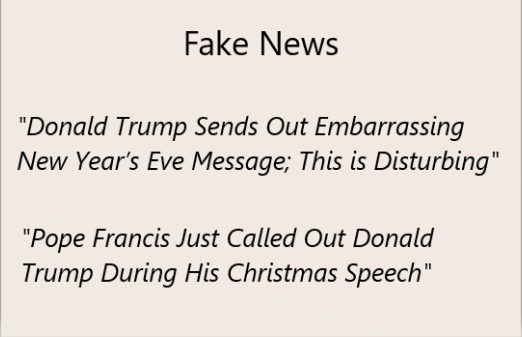
\includegraphics[width=2.5in]{pictures/FakeNews.png}
    \caption{Example of fake news}\label{fig:exampleFake}
\end{figure}

\begin{figure}[H]
    \centering
    
\includegraphics[width=2.5in]{pictures/GoodNews.png}
    \caption{Example of good news}\label{fig:exampleGood}
\end{figure}



We observe that for each title there are some differences in the way things are said that contribute to the algorithm classify it either as a fake new or a good new. Being able to evaluate this is the hardest step to the algorithm. Along side this, it is important to have an even number of phrases for good news and fake news. In figure ~\ref{fig:distributionClasses} we can observe that we have an even number of phrases for each of our classes, good news and fake news. This way we can consider that our classes have and homogeneous number of phrases, preventing disparity in the recognition efficiency.
 
\begin{figure}[H]
    \centering
    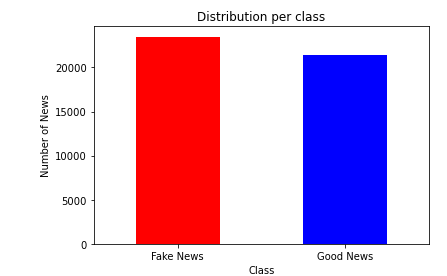
\includegraphics[width=3.5in]{pictures/DistributionClasses.PNG}
    \caption{Distribution of examples per class}\label{fig:distributionClasses}
\end{figure}

Having a complete data set is important, especially in this context where there are a big number of ways that a news could be written and still be fake. However, it is often not enough for the algorithm to obtain good results. Besides this, it is needed to have other techniques to tackle this issue. In the next section, we talk about our approach to obtain better results through pre-processing data mechanisms.

\section{Pre-processing Data}
\subsection{Description}

We already stated that we were using a data set with over 44000 news, and so it is crucial to have some sort of pre-processing mechanisms that increase the effectiveness of the algorithm. Data that is pre-processed in the right way is a major step for higher performances and this step should be a first approach to increase the accuracy of the algorithm. To tackle this problem, we started by transforming text into tokens text since "tokens are the building blocks of Natural Language" \cite{W}. Tokenization is a crucial task in Natural Language Processing. In second place, since tokens remain as text, we encoded them into a sequence of integers. In the next subsections there are further explanations about these mechanisms.

\subsection{Tokenization}

We introduced previously that the first mechanism to pre process data was performing a tokenization. It is a crucial step when natural language is involved, since it is through tokens that it is possible to prepare a vocabulary (set of unique tokens).
\linebreak
\tab Creating a vocabulary with the most frequently occurring words is a simple but efficient way of boosting the model performance.
Furthermore, the tokenization type that is chosen, is a step that must be considered. In our case we decided to perform a word tokenization. This is the most common used algorithm. Based on a certain character, that acts as delimiter, it splits the text into individual words. However there are drawbacks associated with this mechanism, being one the major one the Out Of Vocabulary (OOV) words. When testing, there are words that might not be part of the vocabulary and having a complete data set is crucial as a turn around of this problem.

\subsection{Parsing Tokens into Sequence of Numbers \cite{X}}

Although having tokens and therefore a vocabulary, these tokens needed to be parsed into numbers because machine learning algorithms only work with numbers. This is a mandatory step when working with natural language text. To achieve this, we utilized the method "texts to sequence" \cite{Y} from tensorFlow Keras, that consists in the transformation of each text token into a number, taking only the numberOfWords - 1 most used words into account. This resulted in a sequence of numbers for each title, where the token is the number.
Then, we used the method "pad sequences" \cite{Z} from tensorflow Keras. This method adds padding to each sequence of numbers if they are shorter than the given maximum length we defined as 20. Also, if a sequence is bigger than that value it will be truncated to the desired length. This way, all the sequences will end up with the same size.

\subsection{Conclusion}
In summary in this section we analyzed the pre-processing methods needed to work with text data. Getting this done made our algorithm more efficient. Pre-processing data the right way depending on the data set is a major step to obtain better results.




\section{ML Model Description}
Recapitulating, our theme is fake news detection and, therefore, our goal is to classify a news as either true or false. As a result our data science problem is a classification problem and, from our research, two of the most used models for this type of problem are Long Short-Term Memory Neural Networks and One-Dimensional Convolutional Neural Networks. In order to implement both of them in code we made use of the library "Tensorflow" which automates some steps so that it would be faster to develop.

\subsection{Models} In the next subsections we can see the two models that we used to try to solve our problem.

\subsubsection{LSTM Model \cite{U}}
A Long Short-Term Memory Model is a special kind of Recurrent Neural Networks (RNN) which are neural networks that contain an internal state obtained from previous steps and use it to get the needed results. Furthermore, LSTM has three gates so that it can selectively learn, unlearn or retain information from each of the neural network units. Firstly, the Forget Gate decides what information should be to kept from the previous state. Then, the Input Gate decides what information should be added from the current step. Finally, the Output Gate decides the information that should be passed to the next state. Our implementation is heavily inspired in an algorithm published on "kaggle"\cite{S} where our data set is hosted. It is made of 1 Embedded Layer, 1 LSTM Layer and 1 Dense Layer.

\subsubsection{One-Dimensional CNN Model}
A Convolutional Neural Network is a neural network that attempts to extract features from a window of data from its input. In this project, a One-Dimensional CNN was used due to the data being titles and therefore one-dimensional. In this case, the CNN will attempt to extract features from groups of words. Our implementation is heavily inspired in an algorithm in published on "kaggle"\cite{M}. It is made of 1 Embedded Layer, 1 One-Dimensional Convolutional Layer followed by a Global Max Pooling Layer and 2 Dense Layers.

\subsection{Layers} Building our models, we used the following 5 different types of layers:

\subsubsection{Embedding Layer} The Embedding Layer transforms each sequence of number that represents a word into a vector of a given size.

\subsubsection{LSTM Layer} The LSTM layer is the main layer of a Long Short-Term Memory Neural Network and allows to extract sequences from its input maintaining an internal state.

\subsubsection{Dense Layer} The dense layer is a neural network layer in which each of its neurons receives input from all neurons of the previous layer. This makes it so that it can also be used as an output layer.

\subsubsection{Convolutional Layer} The Convolutional layer is the main layer of a Convolutional Neural Network and allows to extract features from sequences of elements, in our case words.

\subsubsection{Global Max Pooling Layer} The Global Max Pooling Layer reduces the size of its input by selecting the maximum of each vector.

\subsection{Activation Function \cite{L} \cite{O}} All our layers with the exception of the last Dense Layer in each model (which acts as the Output Layer) use the ReLU activation function. This simple function outputs the value it received if positive and if negative it outputs 0. For the last layer we used the sigmoid activation function. This function receives a real value as an input and outputs a value in between 0 and 1.

\subsection{Loss Function \cite{Q}} Both our models use the Binary Crossentropy loss function. The loss value resulting of this function increases as the probability the model outputs for the right class decreases.

\subsection{Optimizer \cite{R}} For our optimizer we decided to use Adam since, from our research, this algorithm combines the advantages of two others. It maintains a per-parameter learning rate (from Adaptive Gradient Algorithm) and the learning rates are obtained from the average of recent magnitudes of the gradients for the weight (from Root Mean Square Propagation).

\section{Model Training}
\subsection{Data Splitting}

In a previous section we talked about our data set and affirmed that it contains 44000+ news. In this section we explain how we split these data into different sets that have different goals. We split data into two sets - Train, Test - that as said before, have different purposes towards helping our models. Next we will explain in more detail which one of this sets as well as a more in depth analysis about their goals.
\linebreak
\tab The \textbf{Train} set consists in a set with 80\% of the original data set. This set has a considerable big percentage in comparison to the other set, because this set is the one that the model will use to train. The standard distribution consists in a share of 60\% to the training set, 20\% to the validation set and finally 20\% for to the testing set. However, as we decided to use k-fold cross validation(which will be explained below) the percentage that was assigned to the validation set was reassigned to the training set.

The \textbf{Test} set consists of the remaining 20\% of the original data set. This set is made of phrases that the model has never seen before and serves the purpose of testing it after the model training is complete. Even tho it contains only 20\% of the origin set, it is considered to be a sufficient number to train variations that might occur in the way the phrases are structured and said.

\subsection{K-Fold Cross Validation \cite{A} \cite{E}}
In the previous section we introduced the concept of k-fold cross validation. Analyzing in depth this technique it can be defined as a procedure used to evaluate machine learning hyper parameters of a model on a limited data sample. In K-Fold CV the associated data set - Train set - is split into a K number of folds where each fold is used as a validation set at some point. For instance, lets imagine the scenario of 4-Fold cross validation(K=4) that was the k parameter we chose in our own project. Here, the data set is split into four folds. In the first iteration, the first fold is used to validate the model and the rest are used to train the model. In the second iteration, the second fold is used as the validation set while the rest serve as the training set. This process is repeated until each fold of the four folds have been used as the validation set. Although in the standard way the data set being divided into 3 data sets - Train, Validation, Test - when using K-fold cross validation we do not have a specific set whose goal is to validate. Instead, the validation set changes, making it so that every fold is used to validate and training, giving rise to more realistic values, unlike the standard way in which the examples of the validation set are static, and may therefore not be realistic. It is because of this that the Train set has 80\%, also encompassing the percentage normally assigned to the validation set.

\subsection{Results}
After making the processes detailed in the previous sections, we then made some graphics to analyse the results. Therefore we can see below, for each model, the confusion matrix, the comparison between training accuracy and cross validation accuracy over the epochs, the comparison between training loss and cross validation loss over the epochs and the accuracy of each class.

\subsubsection{Confusion Matrix}

Below we can see the results regarding confusion matrix of both models.
\linebreak When comparing the LSTM model, represented in figure ~\ref{fig:model1_confmatrix} with the CNN model, represented in figure ~\ref{fig:model2_confmatrix} we can see that they are very similar displaying that both models classified the majority of the data of both classes correctly, presenting slightly better results on the classification of fake news.
\begin{figure}[H]
    \centering
    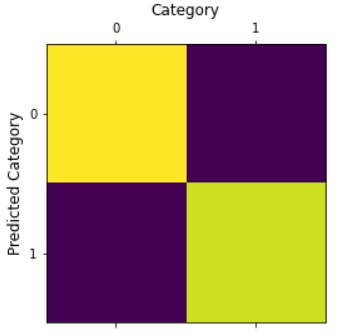
\includegraphics[width=2.5in]{pictures/model1_confmatrix.png}
    \caption{Confusion Matrix (LSTM Model)}\label{fig:model1_confmatrix}
\end{figure}

\begin{figure}[H]
    \centering
    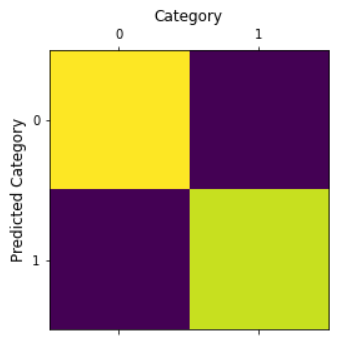
\includegraphics[width=2.5in]{pictures/model2_confmatrix.png}
    \caption{Confusion Matrix (CNN Model)}\label{fig:model2_confmatrix}
\end{figure}

\subsubsection{Model Cross Validation Accuracy and Loss}

Below we can see the results of accuracy and loss regarding both models obtained from Cross Validation.
\linebreak When comparing the LSTM model, represented in the figures ~\ref{fig:model1_accuracy} and ~\ref{fig:model1_loss} with the CNN model, represented in the figures ~\ref{fig:model2_accuracy} and ~\ref{fig:model2_loss} we can see that although both models are very similar in these statistics the LSTM Model still has a bigger validation accuracy and smaller validation loss in comparison to the CNN Model.

\begin{figure}[H]
    \centering
    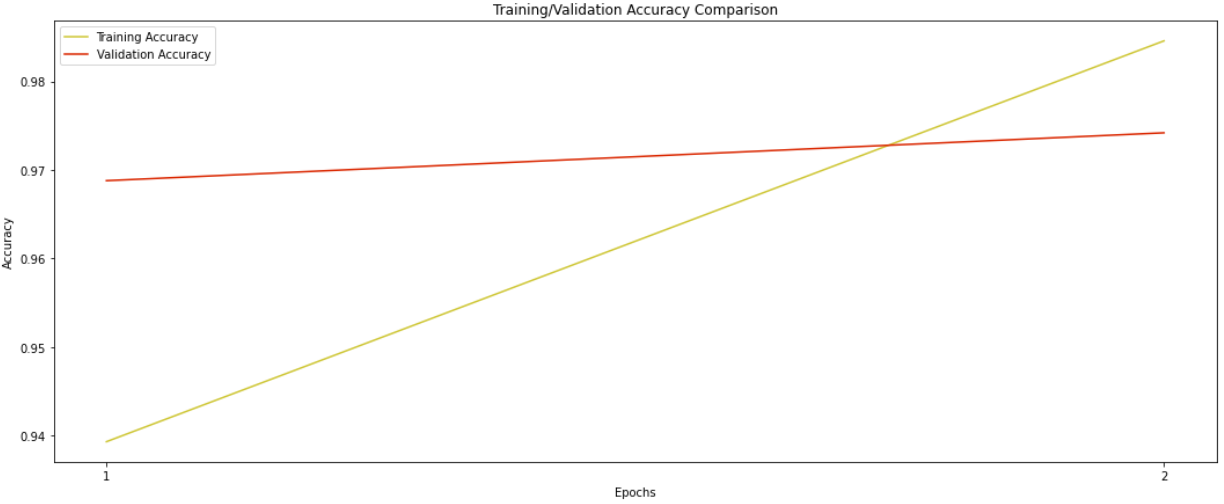
\includegraphics[width=3.5in]{pictures/model1_accuracy.png}
    \caption{Cross Validation Accuracy (LSTM Model)}\label{fig:model1_accuracy}
\end{figure}

\begin{figure}[H]
    \centering
    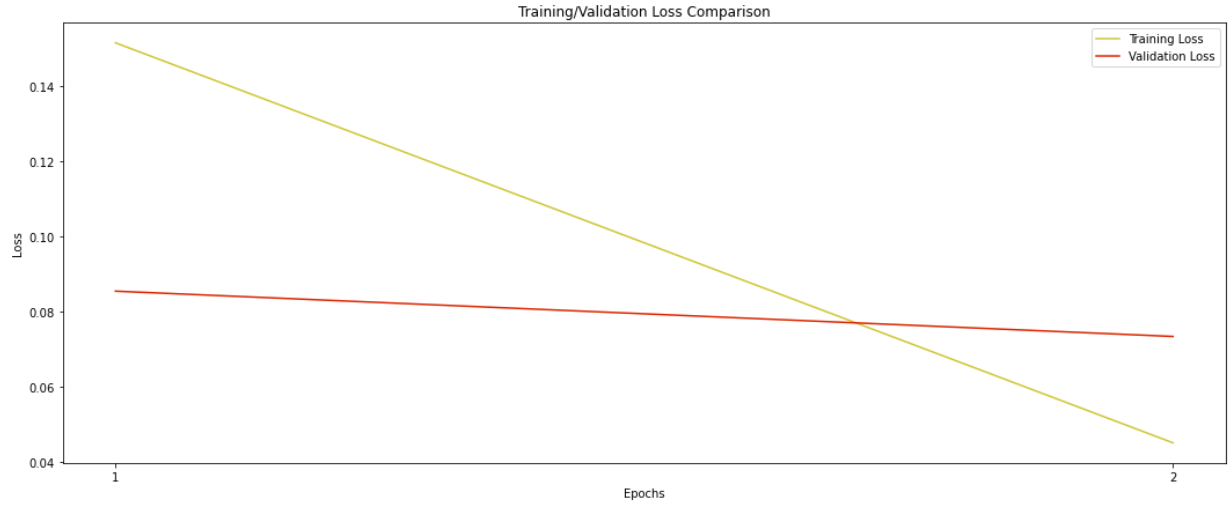
\includegraphics[width=3.5in]{pictures/model1_loss.png}
    \caption{Cross Validation Loss (LSTM Model)}\label{fig:model1_loss}
\end{figure}

\begin{figure}[H]
    \centering
    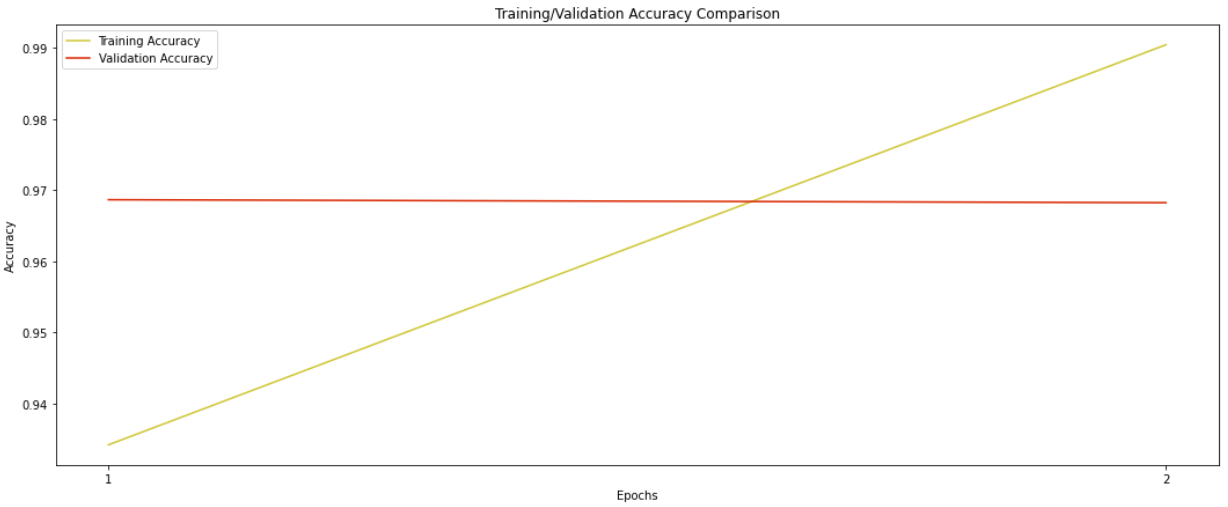
\includegraphics[width=3.5in]{pictures/model2_accuracy.png}
    \caption{Cross Validation Accuracy (CNN Model)}\label{fig:model2_accuracy}
\end{figure}

\begin{figure}[H]
    \centering
    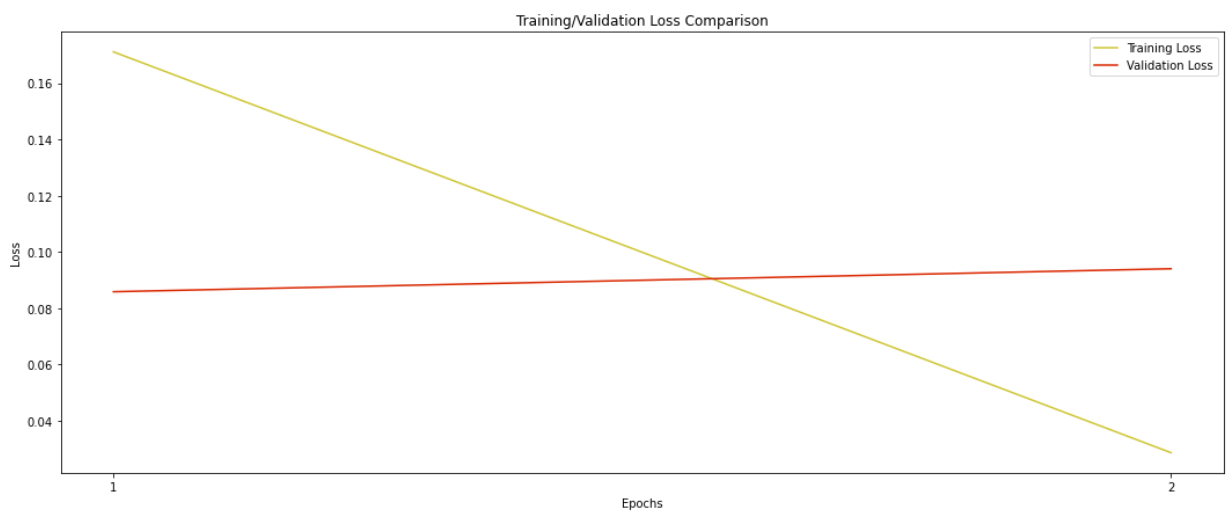
\includegraphics[width=3.5in]{pictures/model2_loss.png}
    \caption{Cross Validation Loss (CNN Model)}\label{fig:model2_loss}
\end{figure}

\subsubsection{Model Number of Parameters}

Below we can see the number of parameters of both models.
\linebreak When comparing the LSTM model, represented in figure ~\ref{fig:model1_parameters} with the CNN model, represented in figure ~\ref{fig:model2_parameters} we can see that both models share the same first embedding layer which accounts for most of the parameters (5000000). Then, excluding that layer both models have a similar number of parameters with LSTM having the most with 60501 parameters and CNN having the least with 48769 parameters.

\begin{figure}[H]
    \centering
    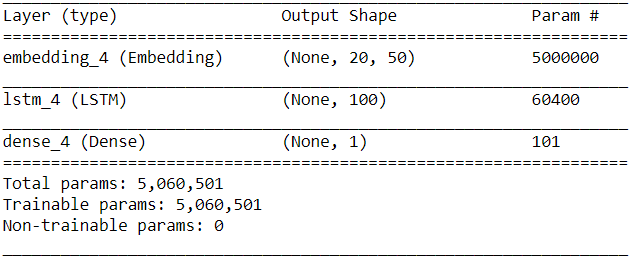
\includegraphics[width=3.5in]{pictures/model1_parameters.png}
    \caption{LSTM Model Parameters}\label{fig:model1_parameters}
\end{figure}

\begin{figure}[H]
    \centering
    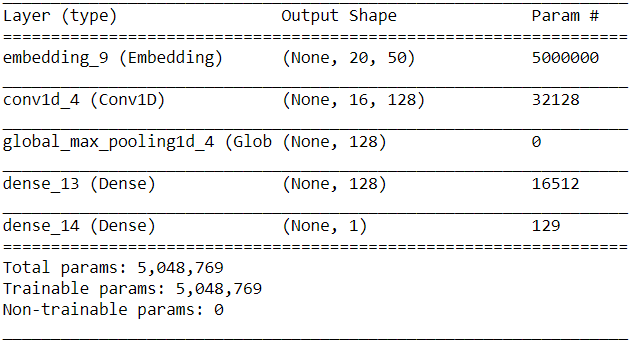
\includegraphics[width=3.5in]{pictures/model2_parameters.png}
    \caption{CNN Model Parameters}\label{fig:model2_parameters}
\end{figure}

\subsubsection{Conclusion}

In table ~\ref{table:comparsion_acc_loss_models} we can compare the 2 algorithms explained in the previous section with the techniques we talked about applied:

\begin{table}[H]
\centering
\caption{Comparison of accuracy and loss of models}
\label{table:comparsion_acc_loss_models}
\begin{tabular}{ | m{7em} | m{2.5cm}| m{2.5cm} | } 
\hline
& LSTM Model & CNN Model \\ 
\hline
Train Accuracy & 0.98630 & 0.9922 \\
\hline
CV Accuracy & 0.9741911441087723 & 0.9705997109413147 \\
\hline
Test Accuracy & 0.9795100092887878 & 0.9733852744102478 \\
\hline
Train Loss & 0.0394 & 0.0236 \\
\hline
CV Loss & 0.07343890331685543 & 0.08617164380848408 \\
\hline
Test Loss & 0.05944212526082992 & 0.07943803817033768 \\
\hline
Precision & 0.98 & 0.97 \\
\hline
Recall & 0.98 & 0.97 \\
\hline
F1 Score & 0.98 & 0.97 \\
\hline
\end{tabular}
\end{table}

As we can see from the results, the LSTM Model obtained the best results in every metric with the exception of the training accuracy and loss. The fact that the CNN Model has higher training statistics might also suggest a greater tendency for it to suffer of over-fitting. Therefore, based on these results the Long Short-Term Memory Model is the best of two.



\section{Hyper-parameters selection}
In previous sections we optimized our model trough a correct data splitting of the data set. Before that we optimized it by doing the correct mechanisms of pre-processing data.In this section, we discuss the effectiveness that different hyper-parameters can offer. These values must not be chosen naively, since they are key to obtain good results.

\subsection{Learning rate}
Starting by understanding the concept behind learning rate \cite{D}, it is defined as "a hyper-parameter that controls how much we are adjusting the weights of our network with respect the loss gradient."
The choice of learning rate must be done the correct way, since it helps with the proper functioning of the model. This value should not be chosen naively and random, but trough methods that test different values and identify the best learning rate. To find the best learning rate, we started by defining a very low value and train the model with this value. In the next iterations this value exponentially grows according to the following equation:
\linebreak

\begin{equation*}
  f(x) = 0,00025 * 2^x , x\geqslant0
\end{equation*}

However the learning rate cannot increase exponentially forever. It must exist a limit where it stops, because the higher the learning rate does not necessarily mean that model obtains better results. In order to define this value, we researched and came to the conclusion that it might be better to not limit the learning rate but the loss it generates. When getting to a certain value of loss, it means that increasing learning rate will only make it worse, and so the optimal learning rate has already been found. In our case we decided to stop on a loss of 0.2.

We applied this method for both of our models, and below we can see the results obtained with the LSTM model. The figures ~\ref{fig:model1_learning_rate_acc} and ~\ref{fig:model1_learning_rate_loss} graphically show the accuracy and loss provided by each learning rate.

\begin{figure}[H]
    \centering
    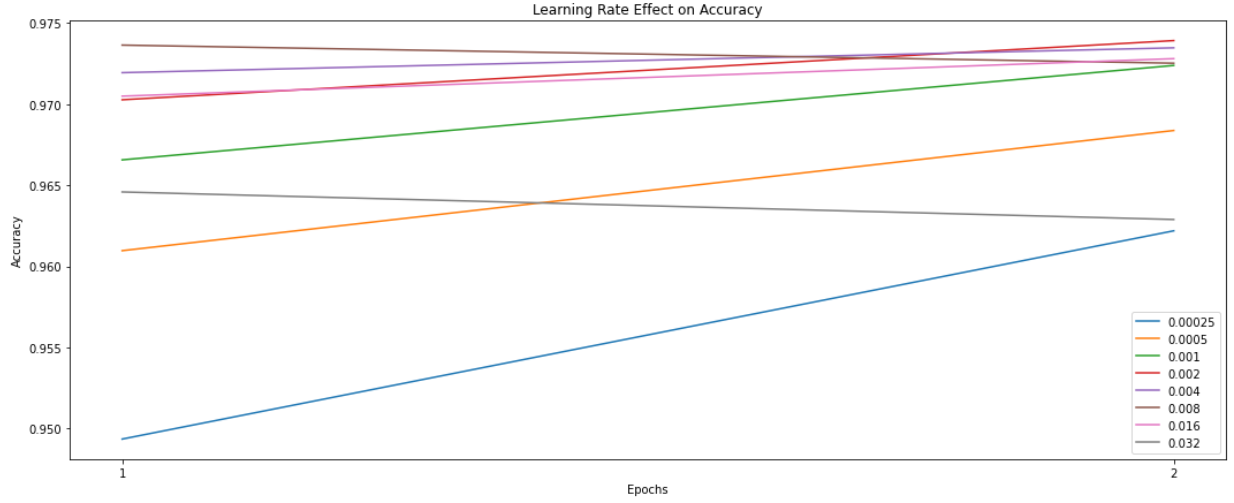
\includegraphics[width=3.5in]{pictures/model1_learning_rate_accuracy.png}
    \caption{Learning Rate effect on Cross Validation Accuracy (LSTM Model)}\label{fig:model1_learning_rate_acc}
\end{figure}

\begin{figure}[H]
    \centering
    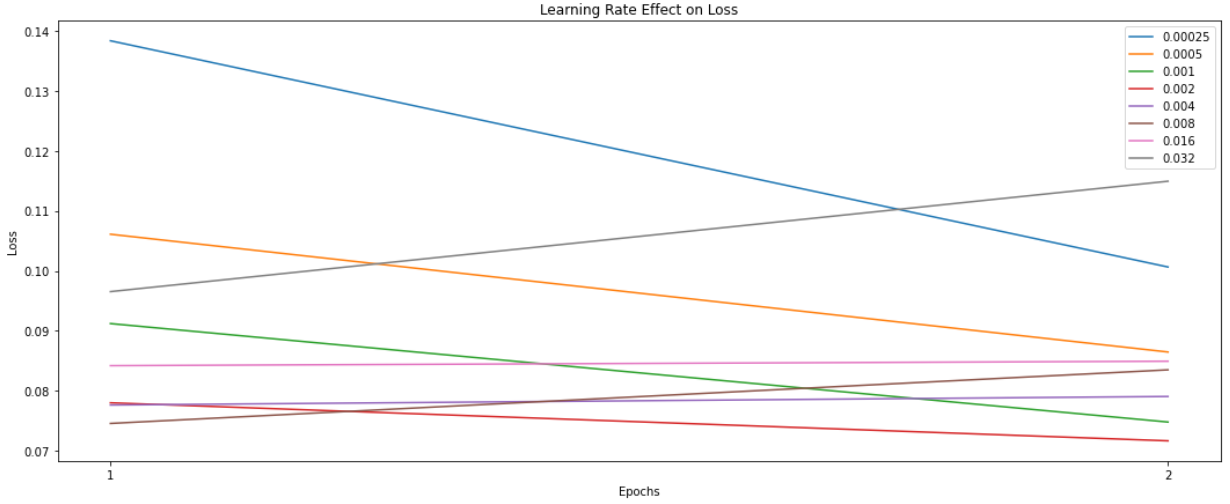
\includegraphics[width=3.5in]{pictures/model1_learning_rate_loss.png}
    \caption{Learning Rate effect on Cross Validation Loss (LSTM Model)}\label{fig:model1_learning_rate_loss}
\end{figure}

\begin{table}[H]
\centering
\caption{Learning rate results on model with 3 Convolutional Layers}
\label{table:model1_learning_rate}
\begin{tabular}{ | m{3.5em} | m{3.2cm}| m{3.2cm} | }
\hline
Learning rate & CV Accuracy & CV Loss \\ 
\hline
0.00025 & 0.9621915221214294 & 0.1006375178694725 \\
\hline
0.0005 & 0.9683722704648972 & 0.0864877812564373 \\
\hline
0.001 & 0.9723814874887466 & 0.0748292151838541 \\
\hline
0.002 & 0.9739127606153488 & 0.07170307449996471 \\
\hline
0.004 & 0.9734672755002975 & 0.07908443920314312 \\
\hline
0.008 & 0.972520649433136 & 0.08351820893585682 \\
\hline
0.016 & 0.9727991223335266 & 0.08495321869850159 \\
\hline
0.032 & 0.9628875404596329 & 0.11491733603179455 \\
\hline
\end{tabular}
\end{table}

Analyzing table ~\ref{table:model1_learning_rate}, we can conclude that a learning rate of 0.002 provides us with a bigger accuracy and a smaller loss therefore it was chosen for this model.


As for the CNN Model, the figures ~\ref{fig:model2_learning_rate_acc} and ~\ref{fig:model2_learning_rate_loss} graphically show the accuracy and loss provided by each learning rate.

\begin{figure}[H]
    \centering
    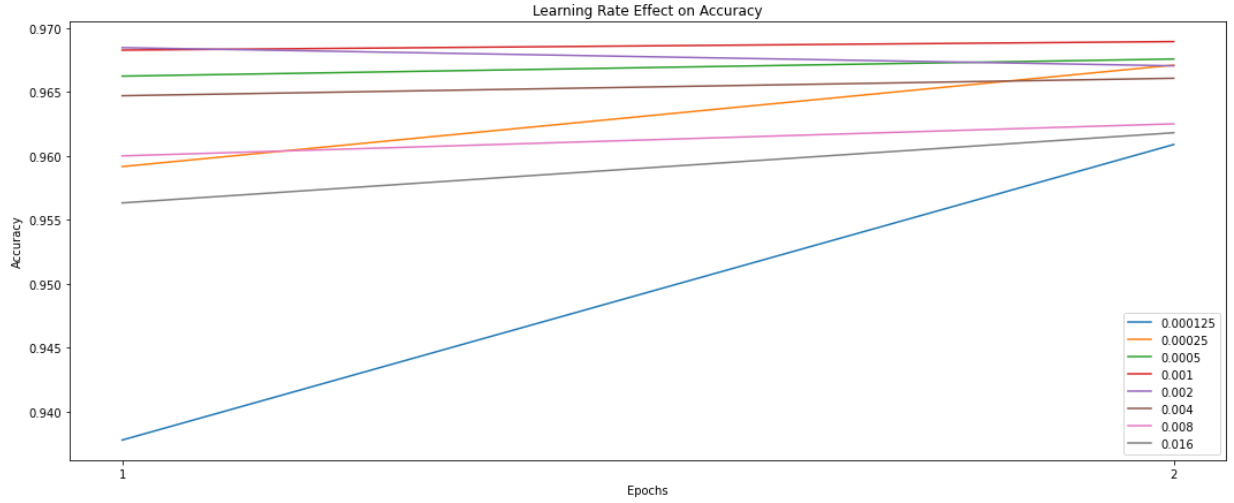
\includegraphics[width=3.5in]{pictures/model2_learning_rate_accuracy.png}
    \caption{Learning rate results on cross Validation Accuracy (CNN Model)}\label{fig:model2_learning_rate_acc}
\end{figure}

\begin{figure}[H]
    \centering
    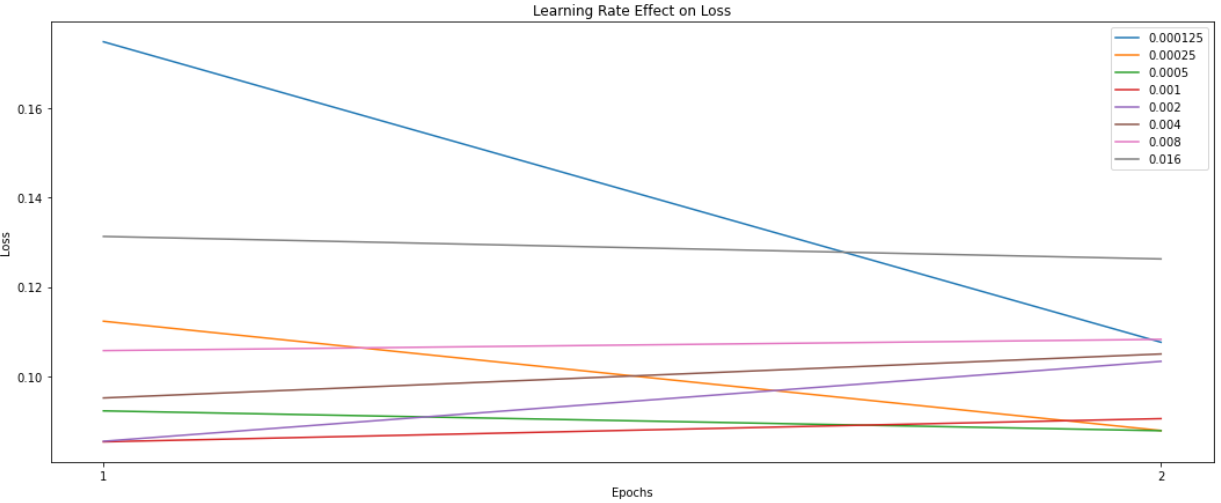
\includegraphics[width=3.5in]{pictures/model2_learning_rate_loss.png}
    \caption{Learning rate results on cross Validation Loss (CNN Model)}\label{fig:model2_learning_rate_loss}
\end{figure}

\begin{table}[H]
\centering
\caption{Learning rate results on model with 2 Convolutional Layers}
\label{table:model2_learning_rate}
\begin{tabular}{ | m{3.5em} | m{3.2cm}| m{3.2cm} | } 
\hline
Learning rate & CV Accuracy & CV Loss \\ 
\hline
0.000125 & 0.9608830958604813 & 0.10761470347642899 \\
\hline
0.00025 & 0.9670916497707367 & 0.08785810321569443 \\
\hline
0.0005 & 0.9675648361444473 & 0.08780965954065323 \\
\hline
0.001 & 0.9689290821552277 & 0.09051806665956974 \\
\hline
0.002 & 0.9670358002185822 & 0.10333718173205853 \\
\hline
0.004 & 0.9660614132881165 & 0.10498812794685364 \\
\hline
0.008 & 0.9624978750944138 & 0.10826252028346062 \\
\hline
0.016 & 0.9618017077445984 & 0.12625912763178349 \\
\hline
\end{tabular}
\end{table}

Analyzing table ~\ref{table:model2_learning_rate}, we can conclude that a learning rate of 0.001 provides us with a bigger accuracy and one of the smallest losses therefore it was chosen for this model.

\subsection{Epochs number \cite{K}}

The definition of the number of epochs in a machine learning algorithm is an important step that should never be done naively. The wrong number of epochs can cause problems such as over-fitting and under-fitting that will be explained later in this section. To understand these problems, it is important to first understand the definition of an epoch. It is defined as the complete cycle of training the neural network with the training data. After the completion of an epoch, the model will change resulting in better accuracy and better loss values, however it is important to refer that the completion of an epoch can take a very long time as well as the need of big computer resources. Upon this, the correct number of epochs is important both for the algorithm and for an efficient need of computer resources.
\linebreak
\tab The major issue related with the incorrect number of epochs is undoubtedly over-fitting and under-fitting. Over-fitting happens when the model learns the training data perfectly, but does not get similar values with validation set. Under-fitting is the other scenario, it means that the model did not learn the training data good enough. A good model is when this results are between.
When we first run the model, this value is chosen randomly because we cannot now the correct value. But after this, it is important to analyze the accuracy and loss both for the training and validation sets, and based on the model decide when this values are closer. When these values are the closest, it means it is the good number of epochs for the model.

For our LSTM model, we can see in the figures ~\ref{fig:epochsLSTM_acc} and ~\ref{fig:epochsLSTM_loss} that these values are the closest on second epoch. Furthermore, this epoch also presents the biggest accuracy and lowest loss.

\begin{figure}[H]
    \centering
    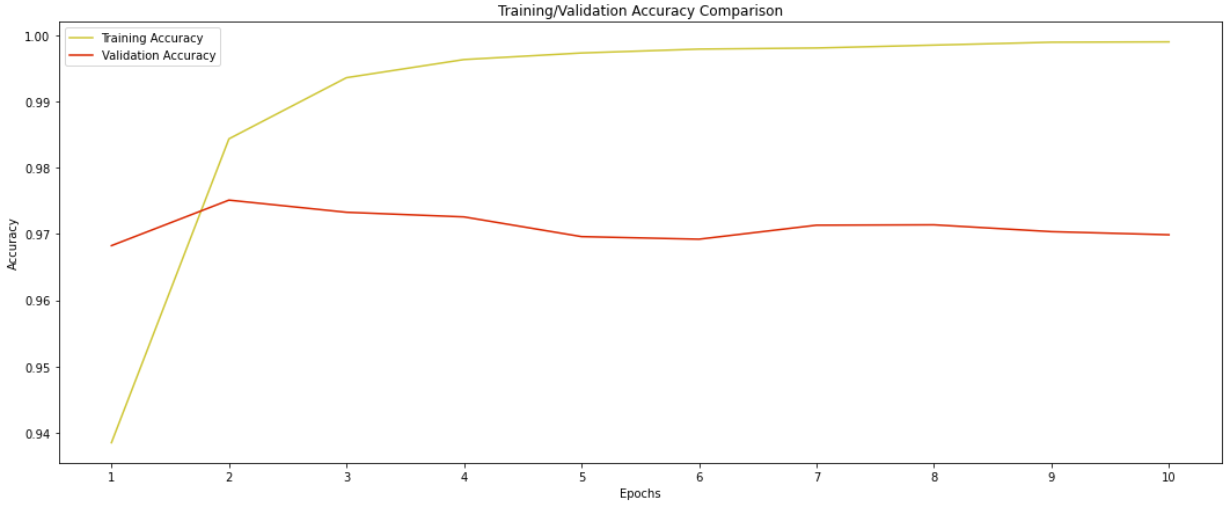
\includegraphics[width=3.5in]{pictures/model1_epochs_accuracy.png}
    \caption{Graphic of accuracy per Epoch (LSTM Model)}\label{fig:epochsLSTM_acc}
\end{figure}

\begin{figure}[H]
    \centering
    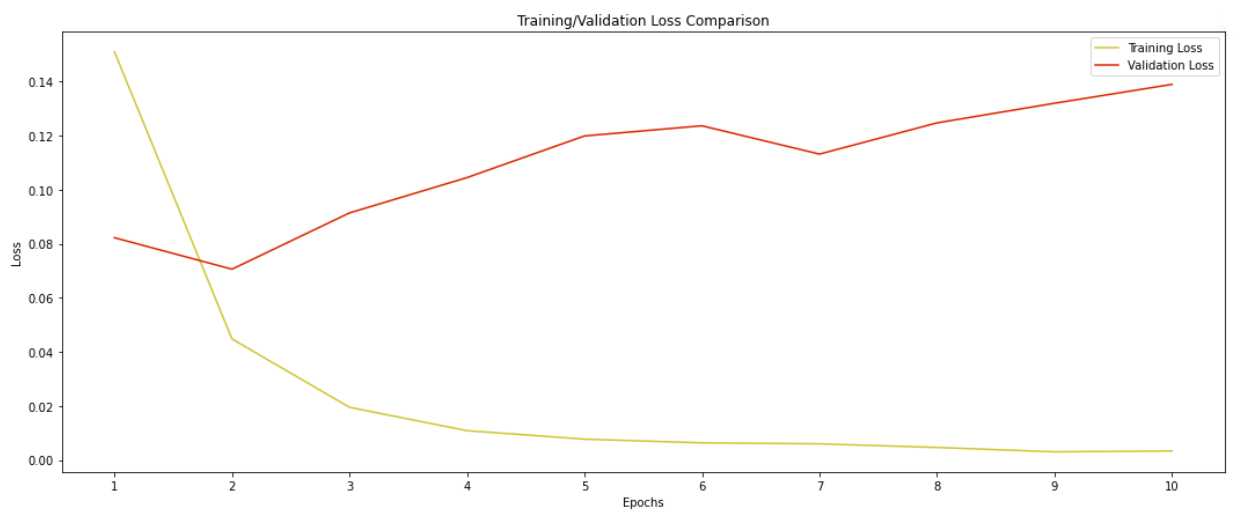
\includegraphics[width=3.5in]{pictures/model1_epochs_loss.png}
    \caption{Graphic of loss per Epoch (LSTM Model)}\label{fig:epochsLSTM_loss}
\end{figure}

For our CNN model, we can see in the figures ~\ref{fig:epochsCNN_acc} and ~\ref{fig:epochsCNN_loss}, that these values also are the closest on the second epoch. Furthermore, this epoch also presents the biggest accuracy and second lowest loss.

\begin{figure}[H]
    \centering
    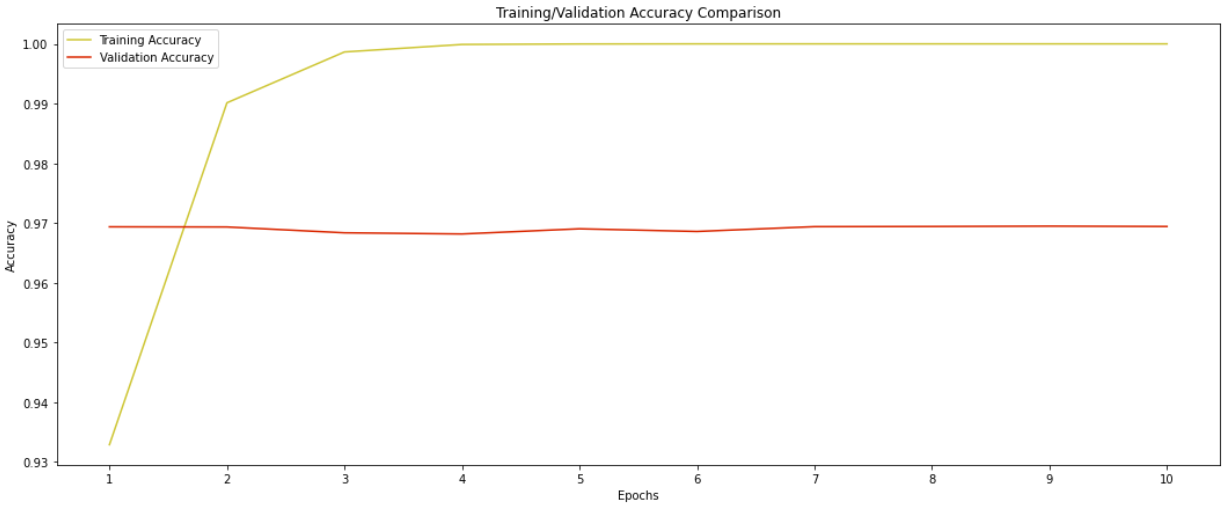
\includegraphics[width=3.5in]{pictures/model2_epochs_accuracy.png}
    \caption{Graphic of accuracy per Epoch (CNN Model)}\label{fig:epochsCNN_acc}
\end{figure}

\begin{figure}[H]
    \centering
    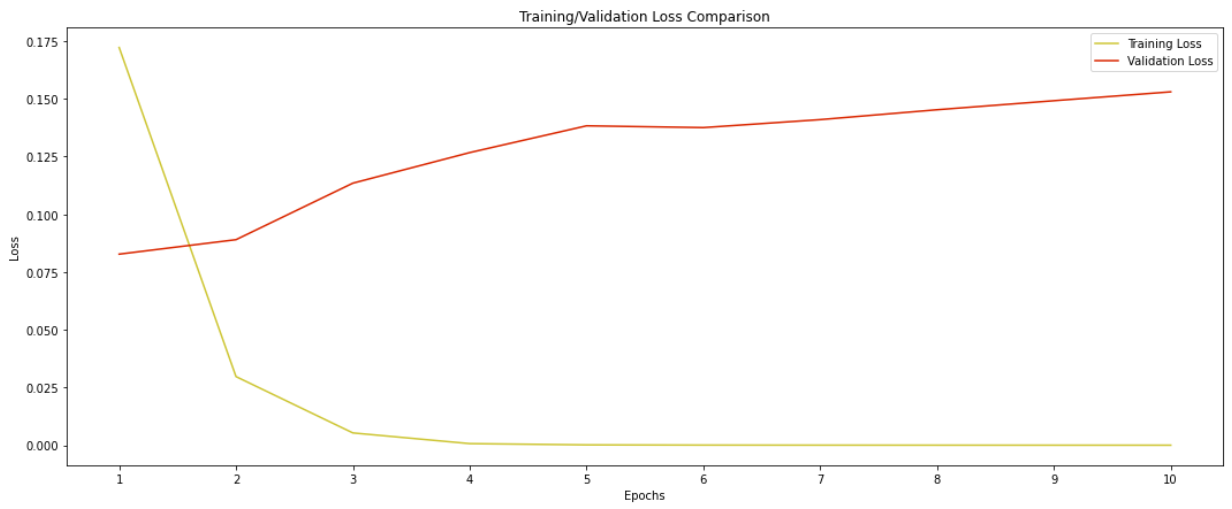
\includegraphics[width=3.5in]{pictures/model2_epochs_loss.png}
    \caption{Graphic of accuracy per Epoch (CNN Model)}\label{fig:epochsCNN_loss}
\end{figure}

Given the previous results, 2 was chosen as the number of epochs for both projects.

\subsection{Dropout Rate \cite{E} \cite{C}}

Dropout is a regularization method where randomly selected nodes are ignored in the model training phase. This nodes are dropped from the model, meaning that they stop contributing to this phase. This regularization method is very interesting and helps in a very common problem in neural networks, which is over-fitting. This problem happens when the model produces an high accuracy in the data that is trained, but when it classifies the values of the test set it does not obtain values as good. That is where dropout and other methods like k-fold cross validation come in handy. Dropout helps fight this issue because encourages the model to learn more sparse data, due to the randomly dropped nodes.

To determine dropout rate, we can see in the figure and table below the values we tested and the conclusions we figured out. Once we only used dropout in the second model, there are only graphics related to this model.

\begin{figure}[H]
    \centering
    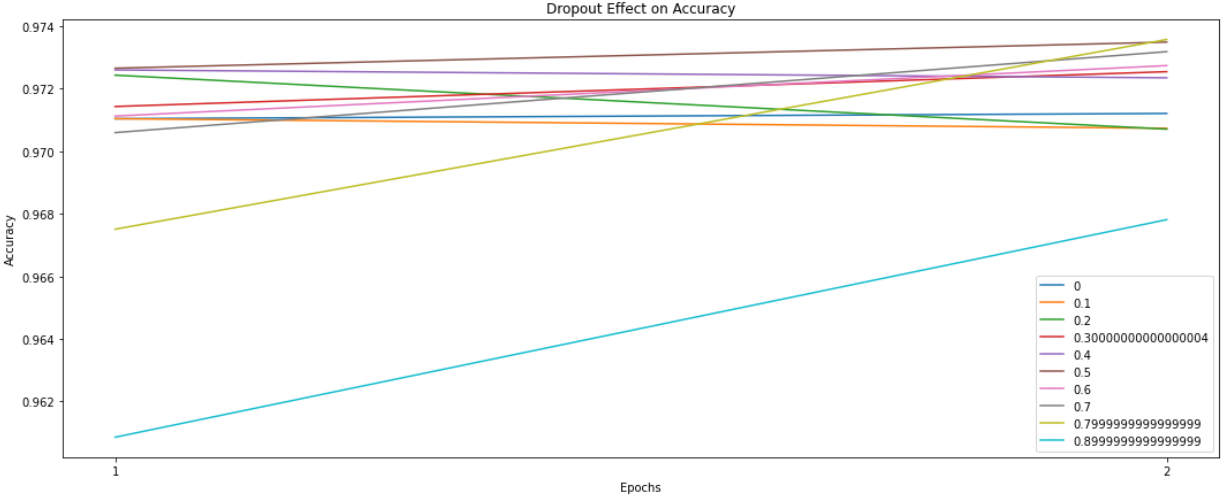
\includegraphics[width=3.5in]{pictures/model1_dropout_accuracy.png}
    \caption{Dropout rate effect on Cross Validation Accuracy (LSTM Model)}\label{fig:dropout_acc}
\end{figure}

\begin{figure}[H]
    \centering
    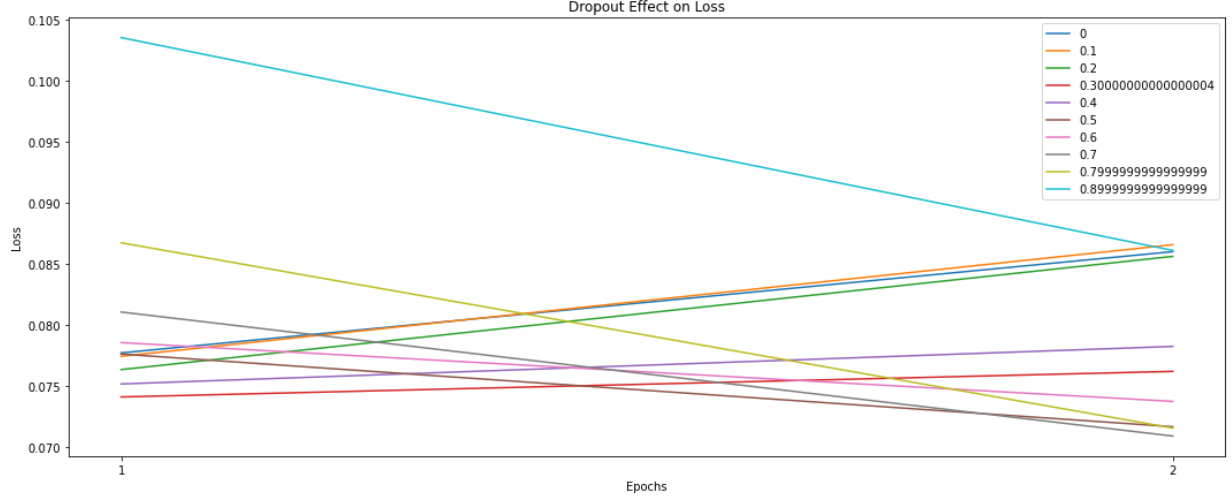
\includegraphics[width=3.5in]{pictures/model1_dropout_loss.png}
    \caption{Dropout rate effect on Cross Validation Loss (LSTM Model)}\label{fig:dropout_loss}
\end{figure}


\begin{table}[H]
\centering
\caption{Dropout results on the LSTM Model}
\begin{tabular}{ | m{3.5em} | m{3.2cm}| m{3.2cm} | } 
\hline
Dropout rate & CV Accuracy & CV Loss \\ 
\hline
0.0 & 0.9712120592594147 & 0.0860103890299797 \\
\hline
0.1 & 0.9707387834787369 & 0.08657958917319775 \\
\hline
0.2 & 0.9707111269235611 & 0.0856237318366766 \\
\hline
0.3 & 0.9725484997034073 & 0.07619954086840153 \\
\hline
0.4 & 0.9723535925149918 & 0.07824386470019817 \\
\hline
0.5 & 0.9734951555728912 & 0.07166404277086258 \\
\hline
0.6 & 0.9727435111999512 & 0.073740528896451 \\
\hline
0.7 & 0.9731889218091965 & 0.07089678756892681 \\
\hline
0.8 & 0.9735786318778992 & 0.07155482657253742 \\
\hline
0.9 & 0.9608553200960159 & 0.08611180633306503 \\
\hline
\end{tabular}
\end{table}

Analyzing these values, we came to the conclusion that the best dropout rate to use is 0.5 given it provides one of the biggest accuracies and one of the lowest losses.

\subsection{Kernel Size}
The kernel size is a hyper-parameter belonging to the Convolutional Layer. It specifies the window size that the convolutional layer will use to extract features from a title. In other words, if we use a kernel size of 3, the layer's extracting window will be 3 word tokens and it will transform all 3 word tokens into a single one. In order to find the best value for this parameter we decided to start with the value 2 since less than that would make convolution impossible and go up until either the cross-validation loss is greater than 0.2 or until it reached 10 which is half the size of the titles inputted.

We applied this method on the CNN model obtaining the results on the figures ~\ref{fig:model2_kernel_size_acc} and ~\ref{fig:model2_kernel_size_loss}, which graphically show the accuracy and loss provided by each kernel size.

\begin{figure}[H]
    \centering
    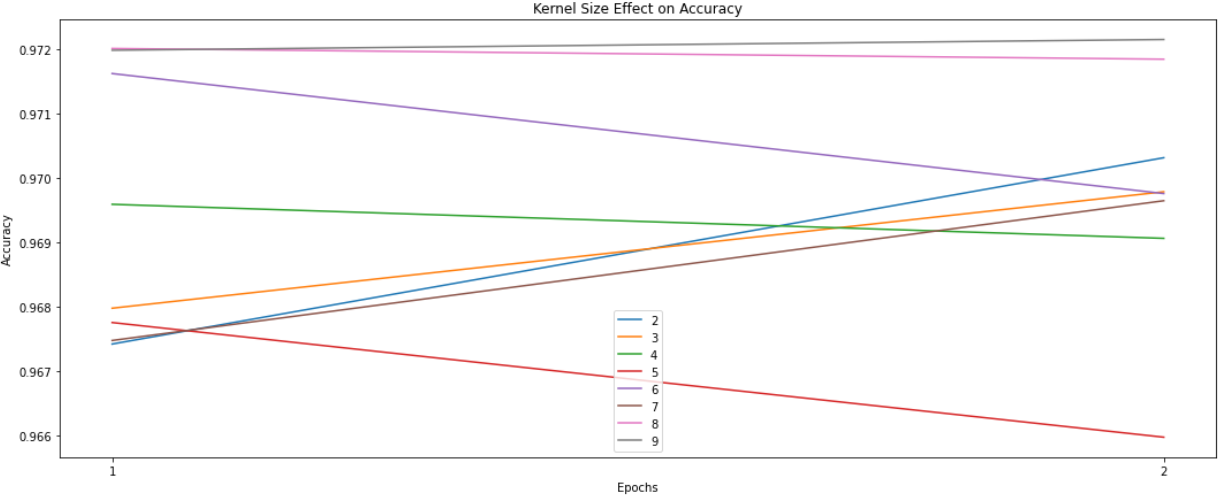
\includegraphics[width=3.5in]{pictures/model2_kernel_size_accuracy.png}
    \caption{Kernel size effects on Cross Validation Accuracy (CNN Model)}\label{fig:model2_kernel_size_acc}
\end{figure}

\begin{figure}[H]
    \centering
    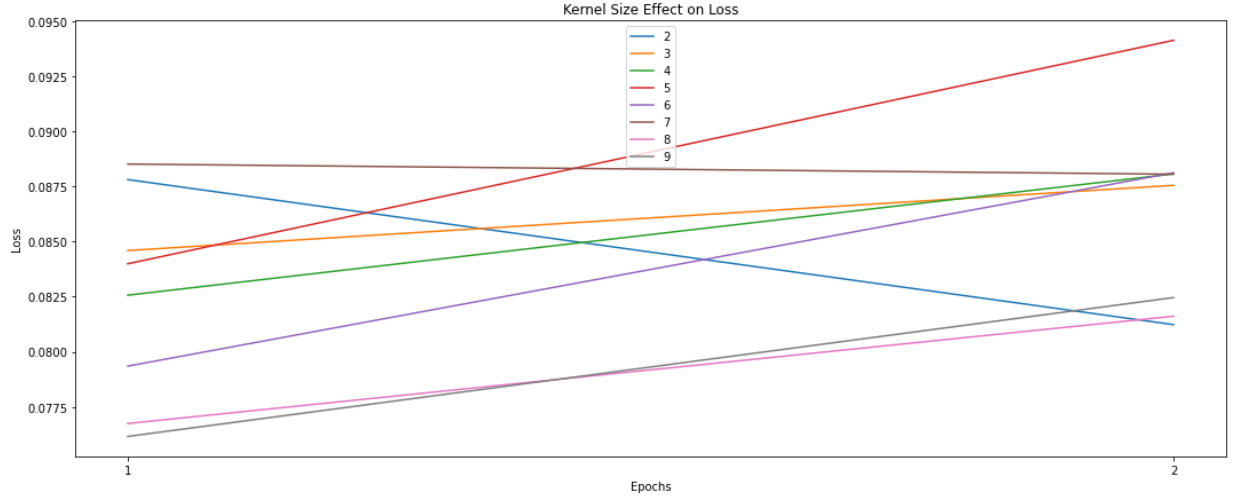
\includegraphics[width=3.5in]{pictures/model2_kernel_size_loss.png}
    \caption{Kernel size effects on Cross Validation Loss (CNN Model)}\label{fig:model2_kernel_size_loss}
\end{figure}

\begin{table}[H]
\centering
\caption{Kernel Size results on the CNN Model}
\label{table:model2_kernel_size}
\begin{tabular}{ | m{2.5em} | m{3.2cm}| m{3.2cm} | }
\hline
Kernel size & CV Accuracy & CV Loss \\ 
\hline
2 & 0.9703213274478912 & 0.08123263157904148 \\
\hline
3 & 0.9697923511266708 & 0.08755910769104958 \\
\hline
4 & 0.9690684527158737 & 0.08807648904621601 \\
\hline
5 & 0.9659779667854309 & 0.09414293244481087 \\
\hline
6 & 0.969764456152916 & 0.08812787011265755 \\
\hline
7 & 0.9696530699729919 & 0.08806292712688446 \\
\hline
8 & 0.9718525409698486 & 0.08161451481282711 \\
\hline
9 & 0.9721588492393494 & 0.08246149308979511 \\
\hline
\end{tabular}
\end{table}

Analyzing table ~\ref{table:model2_kernel_size}, we can conclude that all kernel sizes evaluated presented good results. However, 8 provided us with a bigger accuracy and the second smallest loss therefore it was chosen for this model.

\subsection{Other hyper-parameters}
There are other hyper parameters that could be chosen, throughout methods. However due to the lack of computational power to try different values, for instance, a normal computer cannot process high values in the parameter units from the dense layer. Rather than trying different values chosen by methods, we came to the conclusion that it would be more effective to research in articles and algorithms the most commonly used values. This way we decided upon the following values:

\begin{table}[H]
\centering
\caption{Parameters values}
\begin{tabular}{ | m{7em} | m{1cm} | } 
\hline
Hyper-parameter & Value\\
\hline
LSTM units & 100 \\
\hline
Conv1D filters & 128\\
\hline
Strides & 1 \\
\hline
Dense units & 128 \\

\hline
\end{tabular}
\end{table}

In summary, the choice of hyper-parameter values is necessary and must be made strictly. It must be done through methods rather than be chosen through naive approaches. When chosen correctly, these values can drastically improve the accuracy depending on the previously chosen values.

\section{Comparison with Previous Work}
In this section we plan to compare our work with work that has already been done by other authors. As said previously, our first model is heavily inspired in a LSTM model found in "kaggle" but we managed to obtain better results after our optimizations. While the author of that model obtained an accuracy around 95\% we obtained one around 98\%. Then, our second model is heavily inspired in a CNN model also found in "kaggle" but originally it was being used on all of the text of the news, which we did not do for performance reasons being therefore harder to compare.
\linebreak
\tab When comparing our values with some models we found out in our research \cite{I}, we can see that the best values were 98\% in precision, 100\% in recall and 98\% in F1-score. In our case we have got 98\% in those 3 fields, and our model outperformed all of the other models apart from one. However, this values cannot be truly comparable since the data sets utilized were different.

\section{Conclusions}
With this project we managed to create 2 models to detect fake news. Although we obtained positive results with 98,0\% in test accuracy and 97,4\% in cross-validation accuracy, we believe it is possible to improve them. For example, if we had analysed the text as well as the title we would have more content on which we could have based ourselves on. Also, our data set included a news subjects but none of those subjects existed in both fake and true news, making it a useless information which could have been useful otherwise. Another limitation we faced was the lack of computing power to test some of the parameters (as referred in the previous section) and also to test more complex models.
\linebreak
\tab In summary, through this report we analysed the pre-processing of data and how it impacts the neural network, we discussed 2 models of deep neural networks and how to train and optimize them. We also seen how a neural network can help in real life situations, especially the detection of fake news.
\linebreak
\tab Laslty, it is important to mention that for division of work we consider that both students worked the same amount, as most of the time we were together via zoom.
\begin{flushleft}
- Pedro Amaral 50\%
\end{flushleft}
- Ricardo Cruz 50\%


%------- CITATIONS ----------
\nocite{}
\bibliography{references}
\bibliographystyle{IEEEtran}

\nocite{B}
\nocite{A}
\nocite{D}
\nocite{F}
\nocite{C}
\nocite{H}
\nocite{E}
\nocite{G}
\nocite{I}
\nocite{J}
\nocite{L}
\nocite{N}
\nocite{O}
\nocite{P}
\nocite{Q}
\nocite{R}
\nocite{S}
\nocite{T}

\end{document}


